\section{Relationship to the course (3 to 4 pages) NEEDS DIFFERENT TITLE IS UGLY}
% Summarize the themes/aspects from the lecture course which are relevant for the paper which you will discuss. 
% 
% 
% 
\subsection{Transistors}

The ability to on a large scale produce transistors has been one of the biggest advancements in the 20th century. Transistors and derived devices are necessary components in every modern electronic device. They can amplify currents or switch them off completely. To make these transistors, one needs a material that is capable of showing both characteristics of metals and of insulators, to be able to not only conduct currents, but also switch them off. These materials are called semiconductors, which have a band gap between the valence band and the conduction band. A pure semiconductor material behaves as an insulator, therefore doping of the material is needed to give it the metal-like properties.

\begin{figure}[!ht]
 \begin{center}
  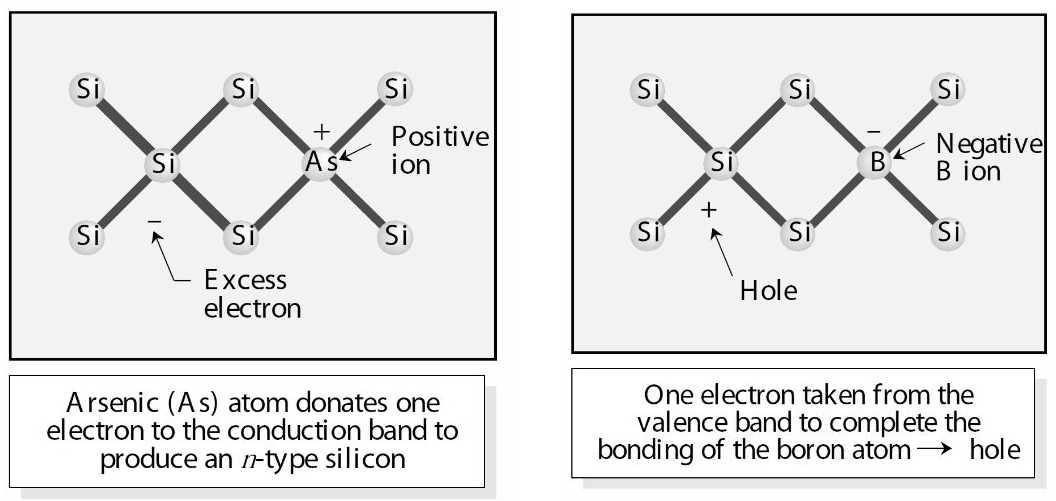
\includegraphics[width=1\textwidth]{doping}
  \caption{N-type doping and p-type doping. From \citet{vanweesbook}.}
  \label{fig:doping}
 \end{center}
\end{figure}

Doping (figure \ref{fig:doping} introduces either extra electrons ($n$-type doping) or extra holes ($p$-type doping) in a material. This is done by putting atoms with different covalent bond forming properties in the crystals. With silicon, which forms 4 covalent bonds, to introduce extra electrons a material which forms 5 covalent bonds (e.g. arsenic) should be used. The extra electron is now free to move. For p-type doping a material that only forms 3 covalent bonds should be used. The `empty' place is a hole which can freely travel through the material.

Field-effect transistors are made of a combination of $n$-type and $p$-type semiconductors. The field effect refers to the control of the electrical conductivity of a material by the application of an external electric field. The working of a junction-FET (JFET) illustrates how this field effect is used.

\begin{figure}[!ht]
 \begin{center}
  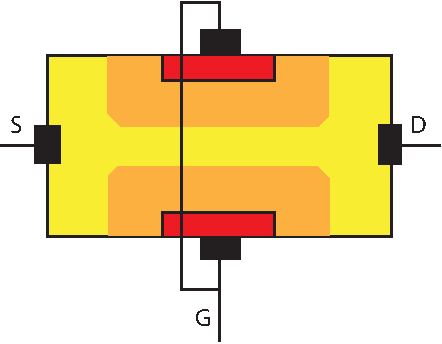
\includegraphics[width=0.7\textwidth]{jfet}
  \caption{A junction field effect transistor, with the position of source, drain and gate shown. Red is the substrate, yellow is the channel. Orange is the depletion zone influenced by the gate voltage.}
  \label{fig:JFET}
 \end{center}
\end{figure}

In figure \ref{fig:JFET} a diagram of a JFET is shown. In this example the channel through which the charge carriers flow (with a voltage difference between source and drain), is made of an $p$-type semiconductor, and the surrounding substrate is made of a $n$-type semiconductor. Therefore the mobile charge carriers in the channel are holes. When the mobile electrons in the substrate are pulled away by a negative voltage applied to the gate, only the static positive charges remain, which forms the depletion zone. This induces a positively charged electric field, which penetrates into the channel and repels the holes there, effectively narrowing the channel. With a high enough gate voltage the channel can be completely `pinched off', resulting in a voltage-controlled switch.

There are other transistor designs that use the field effect in a similar way, a few of which are the MOSFET, MESFET, and the organic OFET. %\textbf{(deze zin mag weg maar verzin dan iets anders afsluitends)}

\subsection{Diodes}
Not only the transistor has had a big impact on society, the field of light-emitting materials has also seen much progress. From indicator lamps to replacements for incandescent light bulbs, the light-emitting diode (LED) has gained a lot of ground.

\begin{figure}[!ht]
 \begin{center}
  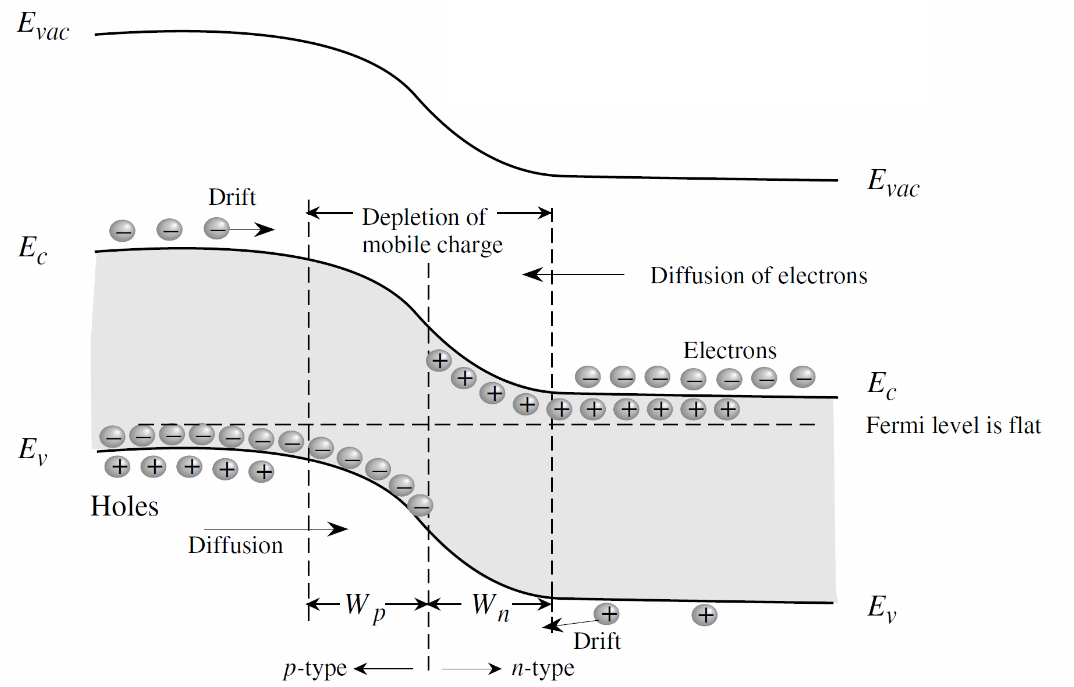
\includegraphics[width=0.8\textwidth]{pn_junction}
  \caption{$p$-$n$ junction. From \citet{vanweesbook}.}
  \label{fig:pn_junction}
 \end{center}
\end{figure}

To make an LED, one needs a $p$-$n$ junction. This is simply a piece of $p$-type semiconductor and $n$-type semiconductor put together. There is a difference in electron and hole densities across the junction, which results in the diffusion of holes from the $p$-side and electrons from the $n$-side. These recombine and near the junction only the static charges remain, which is called the depletion zone. In this region an electric field exists that repels the electrons and holes that enter the region.

If the $p$-type is connected to the positive terminal of a battery, and the $n$-type to the negative terminal (called forward bias), holes from the $p$-side and electrons from the $n$-side are pushed to the depletion zone. The width of the zone is reduced and with enough voltage difference the electrons and holes can go through the depletion zone and recombine with the charge carriers on the other side. Photons with the energy of the band gap of the materials are emitted. This is called electroluminescence and is the basis for an LED.

\subsection{LETs}

A light-emitting field-effect transistor (LET) is a device that couples the electrical characteristics of a FET to the controlled radiative recombination of the electrons and holes, which are injected into the channel via the source and drain contacts \citep{Muccini}. As seen in figure \ref{fig:LET}, the LET also has characteristics similar to a LED. Important is that the materials are able to sustain both electron and hole currents and efficient electroluminescence emission, to get a high quantum efficiency.

\begin{figure}[!ht]
 \begin{center}
  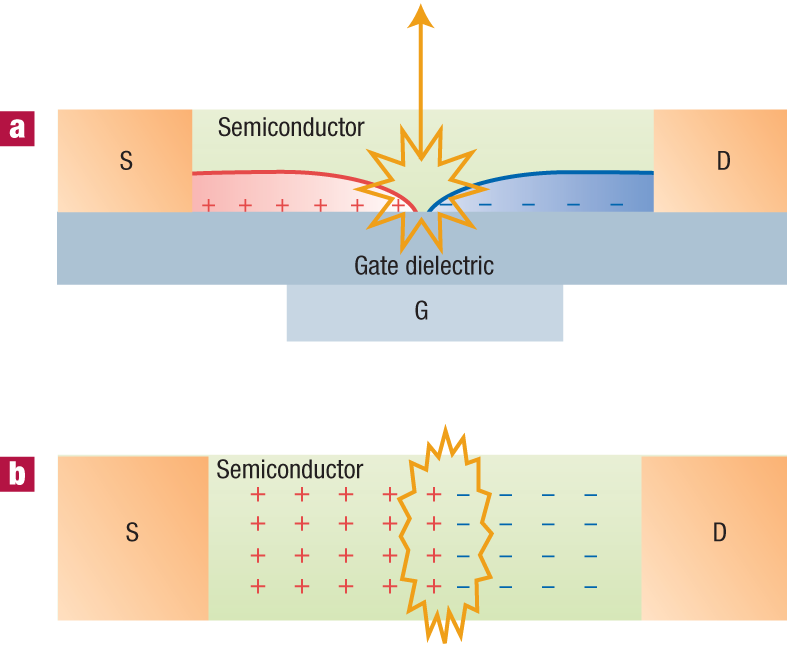
\includegraphics[width=0.6\textwidth]{fig_B1}
  \caption{Scheme of LET. (a) Side view. (b) Top view. The device can be thought of as a sort of forward-biased $p$-$n$ junction. Electrons and holes are injected from the drain (D) and source (S) contacts and recombine within the channel in a position controlled by the gate (G). From \citet{Muccini}.}
  \label{fig:LET}
 \end{center}
\end{figure}


\subsection{Organic Devices}
The previous sections talked about the general structure of different devices, but not much was said about the materials that can be used to make these devices. Only silicon was talked about, however, there are many other suitable materials.


The Organic and optoelectronic part of the lecture is of most relevance to the paper. After the introduction into (inorganic) Light Emmitting Transistors the paper focuses on organic devices.  \citep{loinotes}

\subsubsection{Tuneability}
One of the aspects from the lectures that is also covered in the paper is the tunabilty of organic semiconductors. With bulk inorganic semiconductor material it is not possible to change the bandgap a lot. Especially in light producing devices it is necessary to make nanocrystals. These nanocrystal structures are also needed for indirect bandgap meterials like silicon because they need a phonon to complete charge recombination. Without the nanocrystal structure the rocombination will occur via an non-radiative process. For organic semiconductors however it is relativly easy to change the bandgap. Most of the organic materials have a relative complex molecular structure compared to inorganic materials, therefore there are more possibilities to adjust the molecule slightly rusulting in different properties. 
\subsubsection{Easy and low-cost production}
An other advantage of organic semiconductors that is mentioned both in the lectures and in the article are the favorable production methods. Inorganic semiconductors require an expensive and complicated production method. (Iets uitleggen over litografie en etching etc) Organic semiconductors on the other hand can be easily printed from a solution. The solution can be printed on many different types of (cheaper) materials such as, glass, metal foils and plastics, which give the possibility of producing flexible semiconductors. Finally the costs of the organic semiconductor material itself is much cheaper and more widely available.
\subsubsection{Other differences}
-Mobility of charge

Mentioned briefly in both the paper and lectures is the mobility of charge carriers. For OLEDs the mobility is about 5 orders of magnitude lower than of inorganic LEDs. However the article describes a mobility for OLETs that can be 4 orders of magnitude higher, but still lower than that of inorganic materials.

-Lower efficiency for organic devices

However the efficiency of organic devices continues to increase it still is not at the level of inorganic devices for high brightness. The efficiency of light emitting devices is often described by the quantum efficiency: the ``fraction of excited carriers that recombine radiatively''. The corresponding equation is

\[
 \eta = \frac{R_{r}}{R} = \frac{\tau_{nr}}{(\tau_{tr}+\tau_{nr})},
\]
where $R=$ Total recombination rate, $R_{r}$=Radiative recombination rate, $\tau_{tr}=$Radiative lifetime, $\tau_{nr}=$Non-radiative lifetime. The goal is to have an as high as possible Radiative recombination rate. 

-Lower lifetime and higher vulnerability to the environment for OSC
Finally the lower lifetime of organic semiconductors is mentioned briefly. Organic semiconductors are more vulnorable to the environment because the organic materials react more easily with water or oxygen. Furthermore their lifetime is lower compared to inorganic semicunductors. 
